%%% COMPILE WITH XELATEX, NOT PDFLATEX
\documentclass[letterpaper]{article}
\author{L.M Goodman}
\date{September 2, 2014}
\title{Tezos --- a self-amending crypto-ledger \\ White paper}
%\usepackage[utf8]{inputenc}
%%\setlength{\parskip}{\baselineskip}
\usepackage{amsfonts}
\usepackage{listings}
\usepackage{color}
\usepackage{courier}
\usepackage{epigraph}
\usepackage{fontspec}
\usepackage{newunicodechar}
\usepackage{graphicx}
\usepackage{siunitx}
\usepackage{url}
\usepackage[hidelinks]{hyperref}



%\epigraphfontsize{\small\itshape}
\setlength\epigraphwidth{4.6cm}
\setlength\epigraphrule{0pt}
%\DeclareUnicodeCharacter{42793}{\tz{}}
%\newunicodechar{⚓}{\anchor}
%Ꜩ

\usepackage{url}
\lstset{basicstyle=\footnotesize\ttfamily,breaklines=true}

\newcommand{\tz}{{\fontspec{DejaVu Sans} \small{ꜩ}}}
\begin{document}

\maketitle

\epigraph{\emph{``Our argument is not flatly circular,
but something like it.''}}
{--- \textup{Willard van Orman Quine}}


\begin{abstract}
We present Tezos, a generic and self-amending crypto-ledger. Tezos can
instantiate any blockchain based ledger. The operations of a regular blockchain
are implemented as a purely functional module abstracted into a shell
responsible for network operations. Bitcoin, Ethereum, Cryptonote, etc. can all
be represented within Tezos by implementing the proper interface to the network
layer.

Most importantly, Tezos supports meta upgrades: the protocols can evolve by
amending their own code. To achieve this, Tezos begins with a seed protocol
defining a procedure for stakeholders to approve amendments to the protocol,
\emph{including} amendments to the voting procedure itself. This is not unlike
philosopher Peter Suber's Nomic\cite{Nomic}, a game built around a fully
introspective set of rules.

In addition, Tezos's seed protocol is based on a pure proof-of-stake system
and supports Turing complete smart contracts. Tezos is implemented in OCaml,
a powerful functional programming language offering speed, an unambiguous
syntax and semantic, and an ecosystem making Tezos a good candidate for formal
proofs of correctness.

Familiarity with the Bitcoin protocol and basic cryptographic primitives are
assumed in the rest of this paper.

\end{abstract}
\newpage

\tableofcontents
\newpage

\section{Introduction}
In the first part of this paper, we will discuss the concept of abstract
blockchains and the implementation of a self-amending crypto-ledger.
In the second part, we will describe our proposed seed protocol.

\section{Self-amending cryptoledger}

A blockchain protocol can be decomposed into three distinct protocols:
\begin{itemize}
\item[-] The network protocol discovers blocks and broadcasts transactions.
\item[-] The transaction protocol specifies what makes a transaction valid.
\item[-] The consensus protocol forms consensus around a unique chain.
\end{itemize}

Tezos implements a generic network shell. This shell is agnostic to the
transaction protocol and to the consensus protocol. We refer to the transaction
protocol and the consensus protocol together as a ``blockchain protocol''. We
will first give a mathematical representation of a blockchain protocol and then
describe some of the implementation choices
in Tezos.

\subsection{Mathematical representation}

A blockchain protocol is fundamentally a monadic implementation of concurrent
mutations of a global state. This is achieved by defining ``blocks'' as
operators acting on this global state. The free monoid of blocks acting on the
genesis state forms a tree structure. A global, canonical, state is defined as
the minimal leaf for a specified ordering.

This suggests the following abstract representation:

\begin{itemize}
\item[-]Let $(\mathbf{S},\leq)$ be a totally ordered, countable, set of possible
states.
\item[-]Let $\oslash \notin \mathbf{S}$ represent a special, invalid, state.
\item[-]Let $\mathbf{B} \subset \mathbf{S}^{\mathbf{S} \cup \{\oslash\}}$ be the
set of blocks. The set of \emph{valid} blocks is
$\mathbf{B} \cap \mathbf{S}^{\mathbf{S}}$.
\end{itemize}

The total order on $\mathbf{S}$ is extended so that
$\forall s \in \mathbf{S}, \oslash < s$.
This order determines which leaf in the block tree is considered to be the
canonical one. Blocks in $\mathbf{B}$ are seen as operators acting on the state.

All in all, any blockchain protocol\footnote{GHOST is an approach which orders
the leafs based on properties of the tree. Such an approach is problematic for
both theoretical and practical reasons. It is almost always better to emulate it
by inserting proofs of mining in the main chain.} (be it Bitcoin, Litecoin,
Peercoin, Ethereum, Cryptonote, etc) can be fully determined by the tuple:

$$\left(\mathbf{S},\leq,\oslash,
\mathbf{B} \subset \mathbf{S}^{\mathbf{S} \cup \{\oslash\}}\right)$$

The networking protocol is fundamentally identical for these blockchains.
``Mining'' algorithms are but an emergent property of the network,
given the incentives for block creation.

In Tezos, we make a blockchain protocol introspective 
by letting blocks act on the protocol itself.
We can then express the set of protocols recursively as
$$\mathcal{P} = \left\{\left(\mathbf{S},\leq,\oslash,\mathbf{B} \subset
\mathbf{S}^{(\mathbf{S} \times \mathcal{P})\cup \{\oslash\}} \right)\right\}$$


\subsection{The network shell}
This formal mathematical description doesn't tell us \emph{how} to build the
block tree. This is the role of the network shell, which acts as an interface
between a gossip network and the protocol.

The network shell works by maintaining the best chain known to the client. It is
aware of three type of objects. The first two are transactions and blocks, which
are only propagated through the network if deemed valid. The third are
protocols, OCaml modules used to amend the existing protocol. They will be
described in more details later on. For now we will focus on transaction and
blocks.

The most arduous part of the network shell is to protect nodes against
denial-of-service attacks.

\subsubsection{Clock}
Every block carries a timestamp visible to the network shell. Blocks that appear
to come from the future are buffered if their timestamps are within a few
minutes of the system time and rejected otherwise. The protocol design must
tolerate reasonable clock drifts in the clients and must assume that timestamps
can be falsified.

\subsubsection{Chain selection algorithm}
The shell maintains a single chain rather than a full tree of blocks. This chain
is only overwritten if the client becomes aware of a strictly better chain.

Maintaining a tree would be more parsimonious in terms of network communications
but would be susceptible to denial-of-service attacks where an attacker produces
a large number of low-scoring but valid forks.

Yet, it remains possible for a node to lie about the score of a given
chain, a lie that the client may only uncover after having processed a
potentially large number of blocks. However, such a node can be subsequently
ignored.

Fortunately, a protocol can have the property that low scoring chains exhibit a
low rate of block creation. Thus, the client would only consider a few blocks of
a ``weak'' fork before concluding that the announced score was a lie.

\subsubsection{Network level defense}
In addition, the shell is ``defensive''.
It attempts to connect to many peers across various IP ranges. It detects
disconnected peers and bans malicious nodes.

To protect against certain denial of service attacks, the protocol provides the
shell with context dependent bounds on the size of blocks and transactions.

\subsection{Functional representation}

\subsubsection{Validating the chain}

We can efficiently capture almost all the genericity
of our abstract blockchain structure with the following OCaml types.
To begin with, a block header is defined as:

\lstset{
  language=[Objective]Caml
}
\begin{lstlisting}
type raw_block_header = {
  pred: Block_hash.t;
  header: Bytes.t;
  operations: Operation_hash.t list;
  timestamp: float;
}
\end{lstlisting}

We are purposefully not typing the header field more strongly so it can
represent arbitrary content. However, we do type the fields necessary for the
operation of the shell. These include the hash of the preceding block, a list of
operation hashes and a timestamp. In practice, the operations included in a
block are transmitted along with the blocks at the network level. Operations
themselves are represented as arbitrary blobs.

\begin{lstlisting}
type raw_operation = Bytes.t
\end{lstlisting}

The state is represented with the help of a \textbf{Context} module which
encapsulates a disk-based immutable key-value store. The structure of a
key-value store is versatile and allows us to efficiently represent a wide
variety of states.

\begin{lstlisting}
module Context = sig
   type t
   type key = string list

   val get: t -> key -> Bytes.t option Lwt.t
   val set: t -> key -> Bytes.t -> t Lwt.t
   val del: t -> key -> t Lwt.t
   (*...*)
end
\end{lstlisting}

To avoid blocking on disk operations, the functions use the asynchronous monad
Lwt\cite{LWT}. Note that the operations on the context are purely functional:
\textbf{get} uses the \textbf{option} monad rather than throwing an exception
while \textbf{set} and \textbf{del} both return a new \textbf{Context}.
The \textbf{Context} module uses a combination of memory caching and disk
storage to efficiently provide the appearance of an immutable store.

We can now define the module type of an arbitrary blockchain protocol:

\begin{lstlisting}
type score = Bytes.t list
module type PROTOCOL = sig
   type operation
   val parse_block_header : raw_block_header -> block_header option
   val parse_operation :  Bytes.t -> operation option

   val apply :
     Context.t ->
     block_header option ->
     (Operation_hash.t * operation) list ->
     Context.t option Lwt.t

   val score : Context.t -> score Lwt.t
   (*...*)
end
\end{lstlisting}

We no longer compare states directly as in the mathematical model, instead we
project the \textbf{Context} onto a list of bytes using the \textbf{score}
function. List of bytes are ordered first by length, then by
lexicographic order. This is a fairly generic structure, similar to the one used
in software versioning, which is quite versatile in representing various
orderings. 

Why not define a comparison function within the protocol modules? First off it
would be hard to enforce the requirement that such a function represent a
\emph{total} order. The score projection always verifies this (ties can be
broken based on the hash of the last block). Second, in principle we need 
the ability to compare states across distinct protocols. Specific protocol
amendment rules are likely to make this extremely unlikely to ever happen,
but the network shell does not know that.

The operations \textbf{parse\_block\_header} and \textbf{parse\_operation} are
exposed to the  shell and allow it to pass fully typed operations and blocks to
the protocol but also to check whether these operations and blocks are
well-formed, before deciding to relay operations or to add blocks to the local
block tree database.

The apply function is the heart of the protocol:
\begin{itemize}
\item[-]When it is passed a block header and the associated list of operations,
it computes the changes made to the context and returns a modified copy.
Internally, only the difference is stored, as in a versioning system,
using the block's hash as a version handle.
\item[-]When it is only passed a list of operations, it greedily attempts
to apply as many operations as possible. This function is not necessary for the
protocol itself but is of great use to miners attempting to form valid blocks.
\end{itemize}

\subsubsection{Amending the protocol}

Tezos's most powerful feature is its ability to implement protocol capable
of self-amendment. This is achieved by exposing two procedures functions to the
protocol:

\begin{itemize}
\item[-] \textbf{set\_test\_protocol} which replaces the protocol
used in the testnet with a new protocol (typically one that has been adopted
through a stakeholder voter).
\item[-] \textbf{promote\_test\_protocol} which replaces the current
protocol with the protocol currently being tested
\end{itemize}

These functions transform a Context by changing the associated protocol.
The new protocol takes effect when the following block is applied to the chain.

\begin{lstlisting}
module Context = sig
   type t
   (*...*)
   val set_test_protocol: t -> Protocol_hash.t Lwt.t
   val promote_test_protocol: t -> Protocol_hash.t -> t Lwt.t
end
\end{lstlisting}

The \textbf{protocol\_hash} is the \textbf{sha256} hash of a tarball of
\textbf{.ml} and \textbf{.mli} files. These files are compiled on the
fly. They have access to a small standard library but are sandboxed
and may not make any system call.

These functions are called through the \textbf{apply} function of the protocol
which returns the new \textbf{Context}.

Many conditions can trigger a change of protocol. In its simplest version,
a stakeholder vote triggers a change of protocol. More complicated rules
can be progressively voted in. For instance, if the stakeholder desire they
may pass an amendment that will require further amendments to provide a
computer checkable proof that the new amendment respects certain properties.
This is effectively and algorithmic check of ``constitutionality''.

\subsubsection{RPC}
In order to make the GUI building job's easier, the protocol exposes a JSON-RPC
API. The API itself is described by a json schema indicating the types of the
various procedures. Typically, functions such as \textbf{get\_balance} can
be implemented in the RPC.

\begin{lstlisting}
type service = {
  name : string list ;
  input : json_schema option ;
  output : json_schema option ;
  implementation : Context.t -> json -> json option Lwt.t
}
\end{lstlisting}

The name is a list of string to allow namespaces in the procedures. Input and
output are optionally described by a json schema.

Note that the call is made on a given context which is typically a recent ancestor
of the highest scoring leaf. For instance, querying the context six blocks above
the highest scoring leaf displays the state of the ledger with six confirmations.

The UI itself can be tailored to a specific version of the protocol, or generically
derived from the JSON specification.

\section{Seed protocol}
Much like blockchains start from a genesis hash, Tezos starts with a seed
protocol. This protocol can be amended to reflect virtually any blockchain based
algorithm.

\subsection{Economy}

\subsubsection{Coins}
There are initially $\num{10000000000}$ (ten billion) coins, divisible up to two
decimal places. We suggest that a single coin be referred to as a ``tez''
and that the smallest unit simply as a cent. We also suggest to use the
symbol \tz~(\verb!\ua729!, ``Latin small letter tz'') to represent a tez.
Therefore 1 cent = \tz\num{0.01} = one hundreth of a tez.

\subsubsection{Mining and signing rewards}

\paragraph{Principle}
We conjecture that the security of any decentralised currency requires
to incentivize the participants with a pecuniary reward. As explained in the
position paper, relying on transaction costs alone suffers from a tragedy of the
commons. In Tezos, we rely on the combination of a bond and a reward.

Bonds are one year security deposits purchased by miners.
In the event of a double signing, these bonds are forfeited.

After a year, the miners  receive a reward along with their bond to compensate
for their opportunity cost. The security is primarily being provided by the
value of the bond and the reward need only be a small percentage of that value.

The purpose of the bonds is to diminish the amount of reward needed, and perhaps
to use the loss aversion effect to the network's advantage.


\paragraph{Specifics}
In the seed protocol, mining a block offers a reward of \tz\num{512} and
requires a bond of \tz\num{1536}. Signing a block offers a reward of
$32\Delta T^{-1}$ tez where $\Delta T$ is the time interval in minutes between
the block being signed and its predecessor. There are up to 16 signatures per block
and signing requires no bond.

Thus, assuming a mining rate of one block per minute, about 8\% of the initial
money mass should be held in the form of safety bonds after the first year.

The reward schedule implies at most a 5.4\% \emph{nominal} inflation
rate. \emph{Nominal} inflation is neutral, it neither enrishes nor
impoverishes anyone\footnote{In contrast, Bitcoin's mining inflation impoverishes
Bitcoin holders as a whole, and central banking enrishes the financial
sector at the expense of savers}.

Note that the period of a year is determined from the block's timestamps, not
from the number of blocks. This is to remove uncertainty as to the length of
the commitment made by miners. 

\paragraph{Looking forward}
The proposed reward gives miners a 33\% return on their bond.
This return needs to be high in the early days as miners and signers commit
to hold a potentially volatile asset for an entire year.

However, as Tezos mature, this return could be gradually lowered to the
prevailing interest rate. A nominal rate of inflation below 1\% could safely be
achieved, though it's not clear there would be any point in doing so.

\subsubsection{Lost coins}
In order to reduce uncertainty regarding the monetary mass, addresses
showing no activity for over a year (as determined by timestamps)
are destroyed along with the coins they contain.

\subsubsection{Amendment rules}
Amendments are adopted over election cycles lasting $N = 2^{17} = \num{131072}$
blocks each. Given the  a one minute block interval, this is about three
calendar months. The election cycle is itself divided in four quarters of
$2^{15} = \num{32768}$ blocks. This cycle is relatively short to encourage early
improvements, but it is expected that further amendments will increase the
length of the cycle. Adoption requires a certain quorum to be met. This quorum
starts at $Q = 80\%$ but dynamically adapts to reflect the average
participation. This is necessary if only to deal with lost coins.
 
\paragraph{First quarter}
Protocol amendments are suggested by submitting the hash of a tarball of
\verb!.ml! and \verb!.mli! files representing a new protocol. Stakeholders may
approve of any number of these protocols. This is known as ``approval voting'',
a particularly robust voting procedure.

\paragraph{Second quarter}
The amendment receiving the most approval in the first quarter is now subject to
a vote. Stakeholders may cast a vote for, against or can choose to explicitely
abstain. Abstentions count towards the quorum.

\paragraph{Third quarter} If the quorum is met (including explicit abstentions),
and the amendment received $80\%$ of yays, the amendment is approved and
replaces the test protocol. Otherwise, it is rejected.
Assuming the quorum reached was $q$, the minimum quorum $Q$ is updated as such:
$$Q \leftarrow 0.8 Q + 0.2 q.$$

The goal of this update is to avoid lost coins causing the voting procedure to
become stuck over time. The minimum quorum is an exponential moving average of
the quorum reached over each previous election.

\paragraph{Fourth quarter} Assuming the amendment was approved, it will have
been running in the testnet since the beginning of the third quarter.
The stakeholders vote a second time to confirm they wish to promote the test
protocol to the main protocol. This also requires the quorum to be met and an
$80\%$ supermajority.

We deliberately chose a conservative approach to amendments. However,
stakeholders are free to adopt amendments loosening or tightening this policy 
should they deem it beneficial

\subsection{Proof-of-stake mechanism}

\subsubsection{Overview}

Our proof-of-stake mechanism is a mix of several ideas, including
Slasher\cite{Slasher}, chain-of-activity\cite{CoA}, and proof-of-burn.
The following is a brief overview of the algorithm, the components of which
are explained in more details below.

Each block is mined by a random stakeholder (the miner) and includes
multiple signatures of the previous block provided by random 
stakeholders (the signers). Mining and signing both offer a small reward but
also require making a one year safety deposit to be
forfeited in the event of a double mining or double signing.

The protocol unfolds in cycles of \num{2048} blocks. At the beginning of each
cycle, a random seed is derived from numbers that block miners chose and committed
to in the penultimate cycle, and revealed in the last. Using this random seed,
a follow the coin strategy is used to allocate migning rights and signing rights
to a specific addresses for the next cycle. See figure \ref{fig:pos_figure}.

\begin{figure}[b!]
  \centering
  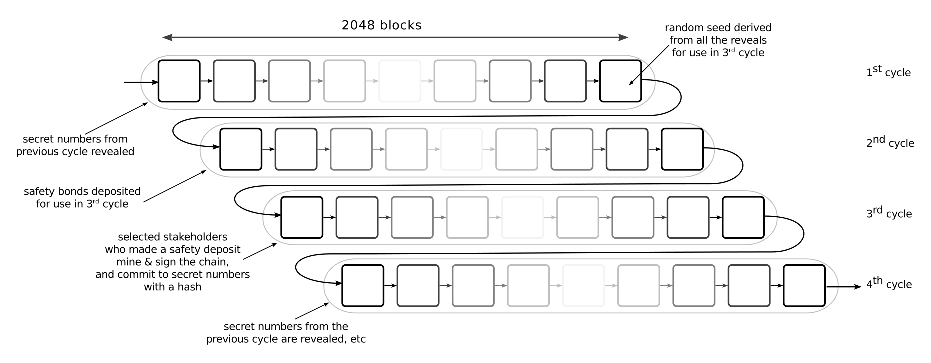
\includegraphics[width=0.8\textwidth]{pos_figure.eps}
  \caption{Four cycles of the proof-of-stake mechanism}
  \label{fig:pos_figure}
\end{figure}


\subsubsection{Clock}

The protocol imposes minimum delays between blocks. In principle, each block
can be mined by any stakeholder. However, for a given block, each stakeholder
is subject to a random minimum delay. The stakeholder receiving the highest
priority may mine the block one minute after the previous block. The
stakeholder receiving the second highest priority may mine the block two
minutes after the previous block, the third, three minutes, and so on.

This guarantees that a fork where only a small fraction of stakeholder
contribute will exhibit a low rate of block creation. If this weren't 
the case, a CPU denial of service attacks would be possible by
tricking nodes into verifying a very long chain claimed to have a very high
score.

\subsubsection{Generating the random seed}

Every block mined carries a hash commitment to a random number chosen by the
miner. These numbers must be revealed in the next cycle under penalty of
forfeiting the safety bond. This harsh penalty is meant to prevent selective
whitholding of the numbers which could be sued to attack the entropy of the seed. 

Malicious miners in the next cycle could attempt to censor such reveals, however
since multiple numbers may be revealed in a single block, they are very unlikely
to succeed.

All the revealed numbers in a cycle are combined in a hash list and the seed is
derived  from the root using the \verb!scrypt! key derivation function. The key
derivation should be tuned so that deriving the seed takes on the order of a
fraction of a percent of the average validation time for a block on a typical
desktop PC.

\subsubsection{Follow-the-coin procedure}

In order to randomly select a stakeholder, we use a follow the coin procedure.

\paragraph{Principle}
The idea is known in bitcoin as follow-the-satoshi. The procedures works
``as-if'' every satoshi ever minted had a unique serial number. Satoshis are
implicitly ordered by creation time, a random satoshi is drawn and tracked
through the blockchain. Of course, individual cents are not tracked directly.
Instead, rules are applied to describe what happens when inputs are combined and
spent over multiple output.

In the end, the algorithm keeps track of a set of intervals associated with each
key. Each intervals represents a ``range'' of satoshis.
Unfortunately, over time, the database becomes more and more fragmented,
increasing bloat on the client side.

\paragraph{Coin Rolls}
We optimize the previous algorithm by constructing large ``coin rolls'' made up
of \num{10000} tez. There are thus about one million rolls in existence. A
database maps every roll to its current owner.

Each address holds a certain set of specific rolls as well as some loose change.
When we desire to spend a fraction of a full roll, the roll is broken and
its serial number is sent in a LIFO queue of rolls, a sort of ``limbo''. Every
transaction is processed in a way that minimizes the number of broken rolls.
Whenever an address holds enough coins to form a roll, a serial number is pulled
from the queue and the roll is formed again.

The LIFO priority ensures that an attacker working on a secret fork cannot
change the coins he holds by shuffling change between accounts.

A slight drawback of this approach is that stake is rounded down to the
nearest integer number of rolls. However, this provides a massive improvement
in efficiency over the follow-the-satoshi approach.

While the rolls are numbered, this approach does not preclude the use of 
fungibility preserving protocols like Zerocash. Such protocols can use
the same ``limbo'' queue technique.

\paragraph{Motivation}
This procedure is functionally different from merely drawing a random address
weighted by balance.

Indeed, in a secretive fork, a miner could attempt to control the generation of
the random seed and to assign itself signing and minting rights by creating the
appropriate addresses ahead of time. This is much harder to achieve if rolls
are randomly selected, as the secretive fork cannot fake ownership of certain
rolls and must thus try to preimage the hash function applied to the seed to
assign itself signing and minting rights. 

Indeed, in a cycle of length $N=\num{2048}$, someone holding a fraction $f$ of
the rolls will receive on average $f N$ mining rights, and the effective
fraction received, $f_0$ will have a standard deviation of
$$\sqrt{\frac{1}{N}}\sqrt{\frac{1-f}{f}}.$$

If an attacker can perform a brute-force search through $W$ different seeds,
then his expected advantage is at most\footnote{this is a standard bound
on the expectation of the maximum of W normally distributed variable}
$$\left(\sqrt{\frac{2\log(W)}{N}}\sqrt{\frac{1-f}{f}}\right)fN$$

blocks. For instance, an attacker controlling $f = 10\%$ of the rolls should
expect  to mine about $205$ blocks per cycle. In a secret fork where he attempts
to control the seed, assuming he computed over a trillion hashes, he could
assign itself about $302$ blocks, or about $14.7\%$ of the blocks. Note that:
\begin{itemize}
\item[-] The hash from which the seed is derived is an expensive key derivation
function, rendering brute-force search impractical.
\item[-] To make linear gains in blocks mined, the attacked needs to expend a
quadratically exponential effort.
\end{itemize}  


\subsubsection{Mining blocks}
The random seed is used to repeatedly select a roll. The first roll selected
allows its stakeholder to mine a block after one minute, the second one after
two minutes --- and so on. 

When a stakeholder observes the seed and realizes he can mint a high priority
block in the next cycle, he can make a security deposit.

To avoid a potentially problematic situation were no stakeholder made a 
safety deposit to mine a particular block, after a 16 minutes delay, the
block may be mined without a deposit.

Bonds are implicitely returned to their buyers immediately in any chain
where they do not mine the block.

\subsubsection{Signing blocks}
As it is, we almost have a working proof of stake system.
We could define a chain's weight to be the number of blocks.
However, this would open the door to a form of selfish mining.

We thus introduce a signing scheme. While a block is being minted, the random
seed is used to randomly assign 16 signing rights to 16 rolls. 

The stakeholders who received signing rights observe the blocks being minted and
then submit signatures of that blocks. Those signatures are then included in
the next block, by miners attempting to secure their parent's inclusion in the
blockchain.

The signing reward received by signers is inversely proportional to the time
interval between the block and its predecessor.

Signer thus have a strong incentive to sign what they genuinely believe to be
the best block produced at one point. They also have a strong incentive to agree
on which block they will sign as signing rewards are only paid if the block ends
up included in the blockchain.

If the highest priority block isn't mined (perhaps because the miner isn't
on line), there could be an incentive for signers to wait for a while, just
in case the miner is late. However, other signers may then decide to sign the
best priority block, and a new block could include those signatures, leaving out
the holdouts. Thus, miners are unlikely to follow this strategy.

Conversely, we could imagine an equilibrium where signers panic and start
signing the first block they see, for fear that other signers will do so and
that a new block will be built immediately. This is however a very contrived
situation which benefits no one. There is no incentive for signers to think this
equilibrium is likely, let alone to modify the code of their program to act
this way. A malicious stakeholder attempting to disrupt the operations would only
hurt itself by attempting to follow this strategy, as others would be unlikely
to follow suit.

\subsubsection{Weight of the chain}

The weight is the number of signatures.


\subsubsection{Denunciations}
In order to avoid the double minting of a block or the double signing of a
block, a miner may include in his block a denunciation.

This denunciation takes the form of two signatures. Each minting signature
or block signature signs the height of the block, making the proof of malfeasance quite concise.

While we could allow anyone to denounce malfeasance, there is really no point to
allow anyone else beyond the block miner. Indeed, a miner can
simply copy any proof of malfeasance and pass it off as its own
discovery.\footnote{A zero-knowledge proof would allow anyone to benefit from
denouncing malfeasances, but it's not particularly clear this carries much
benefit.}

Once a party has been found guilty of double minting or double signing,
the safety bond is forfeited.


\subsection{Smart contracts}


\subsubsection{Contract type}
In lieu of unspent outputs, Tezos uses stateful accounts. When those
accounts specify executable code, they are known more generally as
contracts. Since an account is a type of contract (one with no
executable code), we refer to both as "contracts" in full generality.

Each contract has a ``manager", which in the case of an account is 
simply the owner. If the contract is flagged as spendable, the manager
may spend the funds associated with the contract. In addition, each
contract may specify the hash of a public key used to sign or 
mine blocks in the proof-of-stake protocol. The private key may or
may not be controlled by the manager. 

Formally, a contract is represented as:

\begin{lstlisting}
type contract = {
  counter: int; (* counter to prevent repeat attacks *)
  manager: id; (* hash of the contract's manager public key *)
  balance: Int64.t; (* balance held *)
  signer: id option; (* id of the signer *)
  code: opcode list; (* contract code as a list of opcodes *)
  storage: data list; (* storage of the contract *)
  spendable: bool; (* may the money be spent by the manager? *)
  delegatable: bool; (* may the manager change the signing key? *)
}
\end{lstlisting}

The handle of a contract is the hash of its initial content. Attempting
to create a contract whose hash would collide with an existing contract
is an invalid operation and cannot be included in a valid block.

Note that data is represented as the union type.

\begin{lstlisting}
type data =
  | STRING of string
  | INT of int
\end{lstlisting}

where \verb!INT! is a signed 64-bit integer and string is an array of
up to \num{1024} bytes. The storage capacity is limited to \num{16384} bytes,
counting the integers as eight bytes and the strings as their length.

\subsubsection{Origination}

The origination operation may be used to create a new contract, it specifies
the code of the contract and the initial content of the contract's storage. If
the handle is already the handle of an existing contract, the origination is
rejected (there is no reason for this to ever happen, unless by mistake or
malice).

A contract needs a minimum balance of $\tz~\num{1}$ to remain active. If the
balance falls below this number, the contract is destroyed.

\subsubsection{Transactions}

A transaction is a message sent from one contract to another contract, this
messages is represented as:

\begin{lstlisting}
type transaction = {
  amount: amount; (* amount being sent *)
  parameters: data list; (* parameters passed to the script *)
  (* counter (invoice id) to avoid repeat attacks *)
  counter: int;
  destination: contract hash;
}
\end{lstlisting}

Such a transaction can be sent from a contract if signed using the manager's key
or can be sent programmatically by code executing in the contract. When the
transaction is received, the amount is added to the destination contract's
balance and the destination contract's code is executed. This code can make use
of the parameters passed to it, it can read and write the contract's storage,
change the signature key and post transactions to other contracts.

The role of the counter is to prevent replay attacks. A transaction is only
valid if the contract's counter is equal to the transaction's counter. Once a
transaction is applied, the counter increases by one, preventing the transaction
from being reused.

The transaction also includes the block hash of a recent block that the client
considers valid. If an attacker ever succeeds in forcing a long reorganization
with a fork, he will be unable to include such transactions, making the fork
obviously fake. This is a last line of defense, TAPOS is a great system to
prevent long reorganizations but not a very good system to prevent short term
double spending.

The pair (account\_handle, counter) is roughly the equivalent of an unspent
output in Bitcoin.

\subsubsection{Storage fees}

Since storage imposes a cost on the network, a minimum fee of \tz~1 is assessed
for each byte increase in the storage. For instance, if after the execution of
a transaction, an integer has been added to the storage and ten characters have
been appended to an existing string in the storage, then \tz~18 will be withdrawn
from the contract's balance and destroyed. 


\subsubsection{Code}


The language is stack based, with high level data types and primitives and strict
static type checking. Its design is insipired by Forth, Scheme, ML and Cat.
A full specification of the instruction set is available in\cite{language}.
This specification gives the complete instruction set, type system and semantics
of the language. It is meant as a precise reference manual, not an easy introduction.


\subsubsection{Fees}

So far, this system is similar to the way Ethereum handles transaction. However,
 we differ in the way we handle fees. Ethereum allows arbitrarily long programs
to execute by requiring a fee that increases linearly with the program's
executing time. Unfortunately, while this does provide an incentive for one
miner to verify the transaction, it does not provide such an incentive to other
miners, who must also verify this transaction. In practice, most of the
interesting programs that can be used for smart contracts are very short.
Thus, we simplify the construction by imposing a hard cap on the number of steps
we allow the programs to run for.

If the hard cap proves too tight for some programs, they can break the execution
in multiple steps and use multiple transactions to execute fully. Since Tezos is
amendable, this cap can be changed in the future, or advanced primitives can be
introduced as new opcodes.

If the account permits, the signature key may be changed by issuing a signed
message requesting the change.


\section{Conclusion}
We feel we've built an appealing seed protocol. However, Tezos's true potential
lies in putting the stakeholders in charge of deciding on a protocol that they
feel best serves them.


\bibliographystyle{plain}
\bibliography{biblio}

\end{document}
